\documentclass[5p,times,sort&compress]{elsarticle}

\usepackage[utf8]{inputenc}
\usepackage{amsmath}
\usepackage{amssymb}
\usepackage{amsopn}
\usepackage{mathtools}
\usepackage{bm}
\usepackage[table]{xcolor}
\usepackage{textcomp}
\usepackage{float}
\usepackage{placeins}
\usepackage{gensymb}
\usepackage{dblfloatfix}
\usepackage{chemformula}
\usepackage{siunitx}
\sisetup{detect-all}
\DeclareSIUnit{\atpercent}{at.\%}
\DeclareSIUnit{\wtpercent}{wt.\%}
\DeclareSIUnit{\gramforce}{gf}
\DeclareSIUnit{\angstrom}{\protect \text {Å}}
\usepackage{graphicx}
\graphicspath{{../figures/}}
\usepackage[table,dvipsnames]{xcolor}
\definecolor{Gray}{gray}{0.9}
\definecolor{dkgreen}{rgb}{0,0.6,0}
\definecolor{gray}{rgb}{0.5,0.5,0.5}
\definecolor{mauve}{rgb}{0.58,0,0.82}
\usepackage{booktabs}
\usepackage{multirow}
\usepackage{array}
\usepackage{dblfloatfix}
\usepackage{tabularx}
\usepackage{colortbl}
\usepackage{lscape}
%\usepackage{stfloats}
\usepackage{makecell}
 \usepackage{afterpage}
\usepackage{nicematrix}
\usepackage{float}
\usepackage{subcaption}
\usepackage{tikz}
\usetikzlibrary{positioning}
\usepackage{cuted}
\usepackage{hyperref}
\setlength{\abovedisplayskip}{12pt}
\setlength{\belowdisplayskip}{12pt}
\setlength{\abovedisplayshortskip}{12pt}
\setlength{\belowdisplayshortskip}{12pt}
\hypersetup{
    hidelinks,
    breaklinks=true,
    colorlinks=false,
    linkcolor=black,
    citecolor=black,
    urlcolor=black
}
\usepackage{xr-hyper}
\usepackage{listings}
\lstset{frame=tb,
  language=Python,
  aboveskip=3mm,
  belowskip=3mm,
  showstringspaces=false,
  columns=flexible,
  basicstyle={\small\ttfamily},
  numbers=none,
  numberstyle=\tiny\color{gray},
  keywordstyle=\color{blue},
  commentstyle=\color{dkgreen},
  stringstyle=\color{mauve},
  breaklines=true,
  breakatwhitespace=true,
  tabsize=3
}
\usepackage{cleveref}
\usepackage{placeins}
\usepackage{dblfloatfix}

\usepackage{lineno}
%\linenumbers  % Uncomment this for line-numbers

%\journal{Acta Materialia}

\makeatletter
\def\ps@pprintTitle{%
 \let\@oddhead\@empty
 \let\@evenhead\@empty
 \def\@oddfoot{}%
 \let\@evenfoot\@oddfoot}
\makeatother

\newcommand{\argmax}{\operatornamewithlimits{argmax}}
\newcommand{\etal}{\textit{et al.~}}

\newcommand{\dogu}[1]{\textcolor{red}{\textit{Doğu}: #1}}
\newcommand{\brent}[1]{\textcolor{blue}{\textit{Brent}: #1}}
\newcommand{\samuel}[1]{\textcolor{green}{\textit{Samuel}: #1}}

% \renewcommand{\dogu}{}

\begin{document}

\sloppy

\begin{frontmatter}

%\title{Constraint-First Screening of Low-Activation Refractory Alloys via Linear Programming}

%\title{Design of Terminal Compositions for Joinable/FGM-able Alloy System for Fusion Materials}



%\title{Computational Design of a Doubly-Monotonic Functionally Graded Refractory Alloy for the Fusion First Wall}

\title{Computational Design of a Doubly-Monotonic Functionally Graded Refractory Alloy for Fusion First Wall Applications}

\author[1]{Samuel Ifada\texorpdfstring{\corref{cor1}}{}}
\author[1]{Brent Vela}
\author[1]{Do\u{g}uhan Sar\i{}t\"urk}
\author[1]{James Hanagan}
\author[1,2,3]{Raymundo Arr\'oyave}

\affiliation[1]{organization={Department of Materials Science and Engineering, Texas A\&M University},
                city={College Station},
                postcode={77843}, 
                state={TX},
                country={USA}}

\affiliation[2]{organization={J. Mike Walker '66 Department of Mechanical Engineering, Texas A\&M University},
                city={College Station},
                postcode={77843}, 
                state={TX},
                country={USA}}

\affiliation[3]{organization={Wm Michael Barnes '64 Department of Industrial and Systems Engineering, Texas A\&M University},
                city={College Station},
                postcode={77843}, 
                state={TX},
                country={USA}}


%\begin{abstract}
%In alloy design, constraint-driven screening is traditionally performed by a generate-and-filter workflow, in which every candidate composition on a discrete grid is evaluated with a response model and filtered against performance thresholds. This incurs a cost proportional to the full composition grid, even when only a small fraction of candidates satisfy the constraints. Here we present an alternative framework that reformulates screening as a linear-programming (LP) feasibility problem whenever the response model is linear in alloy composition. Under this formulation, the compositions satisfying all screening criteria form a convex polytope on the atomic-fraction simplex, and the feasible compositions are obtained by enumerating the grid points within this polytope directly, rather than by explicit per-composition response evaluation. We demonstrate the approach using FLARE, a linear-in-composition activation model, to identify candidate plasma-facing and structural alloys for a two-material fusion first wall, screening an eleven-element refractory system against activation limits referenced to tungsten and EUROFER97. The LP-defined feasible set reproduces that of the conventional FLARE generate-and-filter workflow exactly, recovering the identical compositions and activation responses while replacing the evaluation of all \(\sim\!3\times10^{7}\) grid candidates with a direct analytical representation of the feasible space. More broadly, the constraint-first LP framework applies to any alloy-screening workflow governed by response models that are linear in composition.
%\end{abstract}

%\begin{keyword}
%linear programming \sep constraint-first screening \sep feasible composition polytope \sep high-throughput alloy design \sep FLARE \sep low-activation refractory alloys
%\end{keyword}

\begin{abstract}

The first wall of a fusion reactor must withstand extreme heat and particle flux at the plasma-facing surface while also carrying structural loads behind it. Tungsten (W) and W-rich alloys have been investigated as candidate plasma-facing materials, while reduced-activation ferritic-martensitic steels such as EUROFER97 are candidates for the structural region. Directly connecting these two alloy families, however, is challenging because of their thermophysical incompatibility and the formation of brittle W–Fe intermetallic phases. A potential solution is to introduce a compositionally graded transition between W-rich and EUROFER-like alloys to suppress intermetallic phase formation and mitigate thermophysical incompatibility. Here, we search for compositionally compatible W-type and EUROFER-type end members together with a continuous graded path between them, subject to phase-stability, property, and low-activation constraints. We identify a nineteen-alloy path forming a tungsten–vanadium substitutional gradient at a constant 5 at.\% rhenium. Along the path, the solidus temperature decreases monotonically from 3449 to 2195 K, while the Pugh ratio increases monotonically from 2.00 to 3.34. Requiring both properties to change monotonically at every compositional step is imposed as a hard constraint, rather than through weighted objectives or tunable penalty parameters.

The path
passes through the small set of compositions satisfying both design criteria, which constitute the only monotone gateway between the two alloy families. This monotonic profile translates directly into a deposition schedule for a prescribed through-wall gradient. The proposed framework is generally applicable to graded-alloy design problems governed by composition-linear screening models.
\end{abstract}

\begin{keyword}
functionally graded alloys \sep fusion first wall \sep
low-activation refractory alloys \sep high-throughput alloy design \sep
graph-based path planning \sep monotonic property gradients
\end{keyword}

\end{frontmatter}

\section{Introduction}

The first wall of a fusion reactor is a two-material system. A plasma-facing
material meets the plasma, withstanding extreme heat flux, particle bombardment,
and neutron irradiation, while a structural alloy behind it carries the mechanical
load. Tungsten leads as the plasma-facing material for its high melting point, low
sputtering yield, and good thermal conductivity, but it is brittle and unsuited to a load-bearing role~\cite{tungstenPFMreview2023}, whereas reduced-activation
ferritic-martensitic steels such as EUROFER97 serve as the structural material
with favorable activation but limited high-temperature
capability~\cite{lindau2005eurofer,RAFMreview2017}. Both must also resist
irradiation damage and remain acceptably activated through operation and
decommissioning~\cite{zinkle2000operating,bloom2007critical}. No single material
satisfies the surface and structural requirements simultaneously, so the first
wall is necessarily built from a plasma-facing material and a structural material
that must somehow be joined into one component.

Joining these materials is a central difficulty. Tungsten and steel differ
markedly in thermal expansion (coefficients of roughly \(4.4\) and
\(12.7 \times 10^{-6}\)~K\(^{-1}\)), so an abrupt joint concentrates large thermal
stresses, and direct tungsten-iron contact forms brittle intermetallics,
principally Fe\(_2\)W and Fe\(_7\)W\(_6\), that embrittle the
joint~\cite{fgmWsteelCGS2022,karim2024wire}. A functionally graded alloy, whose
composition varies continuously from a tungsten-rich plasma-facing terminal to a
structural terminal, can spread the expansion mismatch over a graded region rather
than a single boundary~\cite{fgmWEurofer2015}; such gradients are now
practically realizable, with additive manufacturing routes such as directed
energy deposition able to vary the feed composition layer by
layer~\cite{karim2024wire}. Grading alone, however, does not avoid the intermetallics, since iron and
tungsten still meet across the gradient. The remedy is to keep the transition
a single body-centered cubic (BCC) solid solution at every step, so the path
never enters the composition ranges where the brittle phases are
stable~\cite{fgmWsteelInterlayerBCC2023}. This choice replaces the structural
terminal itself. Rather than grading toward a steel such as EUROFER97, the
gradient terminates in a vanadium-rich structural alloy, low in activation
and reachable from tungsten through a continuous BCC path, so that iron and
tungsten no longer meet along the transition. Finding such a path by
inspection is difficult, since the constraints interact across the
composition space, and existing realizations rely on a few hand-selected
interlayers chosen one composition at a
time~\cite{fgmWsteelInterlayerBCC2023}. Here we instead search the entire
feasible composition space for the graded path directly, so the single-phase
transition is designed rather than assembled from discrete steps.

Designing such a path is a constrained search. The role-specific demands are
divided between the terminals, the plasma-facing side taking the
high-temperature requirement and the structural side the ductility
requirement, but the requirements shared by the whole wall, low activation, a
stable single-phase structure, and adequate thermal conductivity, must be met
by both terminals and every intermediate step alike. Multicomponent
refractory alloys offer wide freedom to balance these
demands~\cite{HEAnuclear2021,Senkov2010}, and high-throughput screening under
multiple simultaneous property constraints has proven effective for
navigating refractory alloy spaces of this kind, combining CALPHAD
thermodynamics with physics-based strength and ductility models to reduce
vast composition spaces to actionable candidate
sets~\cite{vela2023data,HTcalphad2022}. The scale remains demanding, however,
as an eleven-element system on a \(5\)~at.\% grid already spans tens of
millions of compositions, far more than can be tested, and among the
criteria, neutron-induced activation is especially consequential, since
transmutation governs decay heat, dose rates, maintenance, and waste
burden~\cite{RAFMreview2017}, motivating low-activation, radiation-tolerant
elements~\cite{HEAnuclear2021,ElAtwani2019Radiation}.

The First Wall Loading and Activation Response Engine (FLARE) makes the
activation criteria tractable at this scale
\textcolor{red}{\cite{flare}}. Rather than running a full inventory
calculation for every candidate, FLARE precomputes the activation response of
each pure element under a fixed irradiation and decay scenario, so that the
response of any alloy follows as a composition-weighted combination of these
elemental contributions, compared against references such as pure tungsten
and EUROFER97. Because every response is such a weighted combination, the
activation criteria are linear in composition, and the compositions
satisfying all of them form a convex region bounded by the constraint
hyperplanes. Linear programming describes this region directly, so the
feasible space is obtained without evaluating the candidates one by one, and
it is used here as the screening step rather than as the object of the work.

The feasible space is the starting point for the design. Within it, high-throughput
thermodynamic and mechanical evaluation identifies the compositions that are
single-phase, thermally conductive, and suited to the plasma-facing and structural
roles. Treating these compositions as nodes on a simplex lattice, with neighbors
connected by single-step composition changes, turns the design space into a graph
whose connected regions can be traversed~\cite{nimplex}. The two terminals are
located within the largest connected, single-phase region, and the graded path
between them is found as the shortest route through this graph along feasible
neighbors only, which yields the most gradual feasible transition, the fewest
single-step composition changes between terminals. The path is additionally
required to be monotonic in both design properties, with the solidus
temperature never increasing and the ductility never decreasing from the
plasma-facing terminal to the structural terminal, so that no interior layer
of the graded wall is hotter-melting than the layer in front of it or less
ductile than the layer behind it. The same connectivity that
defines the connected feasible regions also supplies the routes between
compositions, so the identification of the design region and the construction of
the graded path follow from a single graph. The path therefore stays single-phase
and activation-feasible at every step and never enters the ranges where brittle
intermetallics would form.

Path planning in composition space has an established lineage in the design of
compositionally graded alloys. Kirk et al.\ introduced a computational
methodology that plans gradient paths through high-dimensional composition
spaces while avoiding undesirable phase regions~\cite{kirk2018gradient}, an
approach subsequently realized experimentally in additively manufactured
gradients~\cite{eliseeva2019fgm}, and later extended the framework to produce
paths with monotonic property profiles, on the argument that a monotonic
gradient can be reshaped into nearly any spatial profile on the part by
controlling the deposition rate~\cite{kirk2021monotonic}. In that work
monotonicity is promoted through a penalized cost function whose weight must
be selected, and it is treated for a single property at a time, with extension
to multiple properties explicitly identified as future
work~\cite{kirk2021monotonic}. Graph representations of composition space
have also been extended, within the same design framework, to multi-terminal
graded structures~\cite{multiterminalCGA2024}, though without property
monotonicity. The graded
first wall poses a harder version of the problem: two properties with opposing
trends, a solidus that must only decrease and a ductility that must only
increase along the same path, with every intermediate composition
simultaneously subject to activation, phase-stability, and conductivity
constraints. To our knowledge, path planning under simultaneous monotonicity
in two opposing properties has not been reported; here it is enforced not
through a tuned penalty but as a hard constraint, by deleting every
property-violating transition from the graph before an exact shortest-path
search.

In this work we design a functionally graded alloy for the fusion first wall in
an eleven-element refractory system \ch{Cr-Fe-Hf-Mo-Nb-Re-Ta-Ti-V-W-Zr}. The
contribution is a doubly-monotonic, single-phase compositional path from a
tungsten-rich plasma-facing terminal to a vanadium-rich structural terminal
that remains activation-feasible throughout, avoiding the brittle
intermetallics that limit conventional tungsten-to-steel graded joints.
Activation screening referenced to tungsten and EUROFER97 defines the feasible
space; thermodynamic and mechanical evaluation reduces it to a connected
single-phase region governed by phase stability, thermal conductivity, solidus
temperature, and ductility; and graph-based path design connects the terminals
through it. To our knowledge, this is the first compositional gradient designed
under simultaneous monotonicity in two opposing properties. The resulting path achieves monotonicity at zero cost in path length,
passing exclusively through the small set of compositions that form the only
monotone gateway between the two categories, and the framework, summarized
in Figure~\ref{fig:overview}, applies generally to graded-alloy design
governed by composition-linear screening models.



\begin{figure*}[!t]
  \centering
  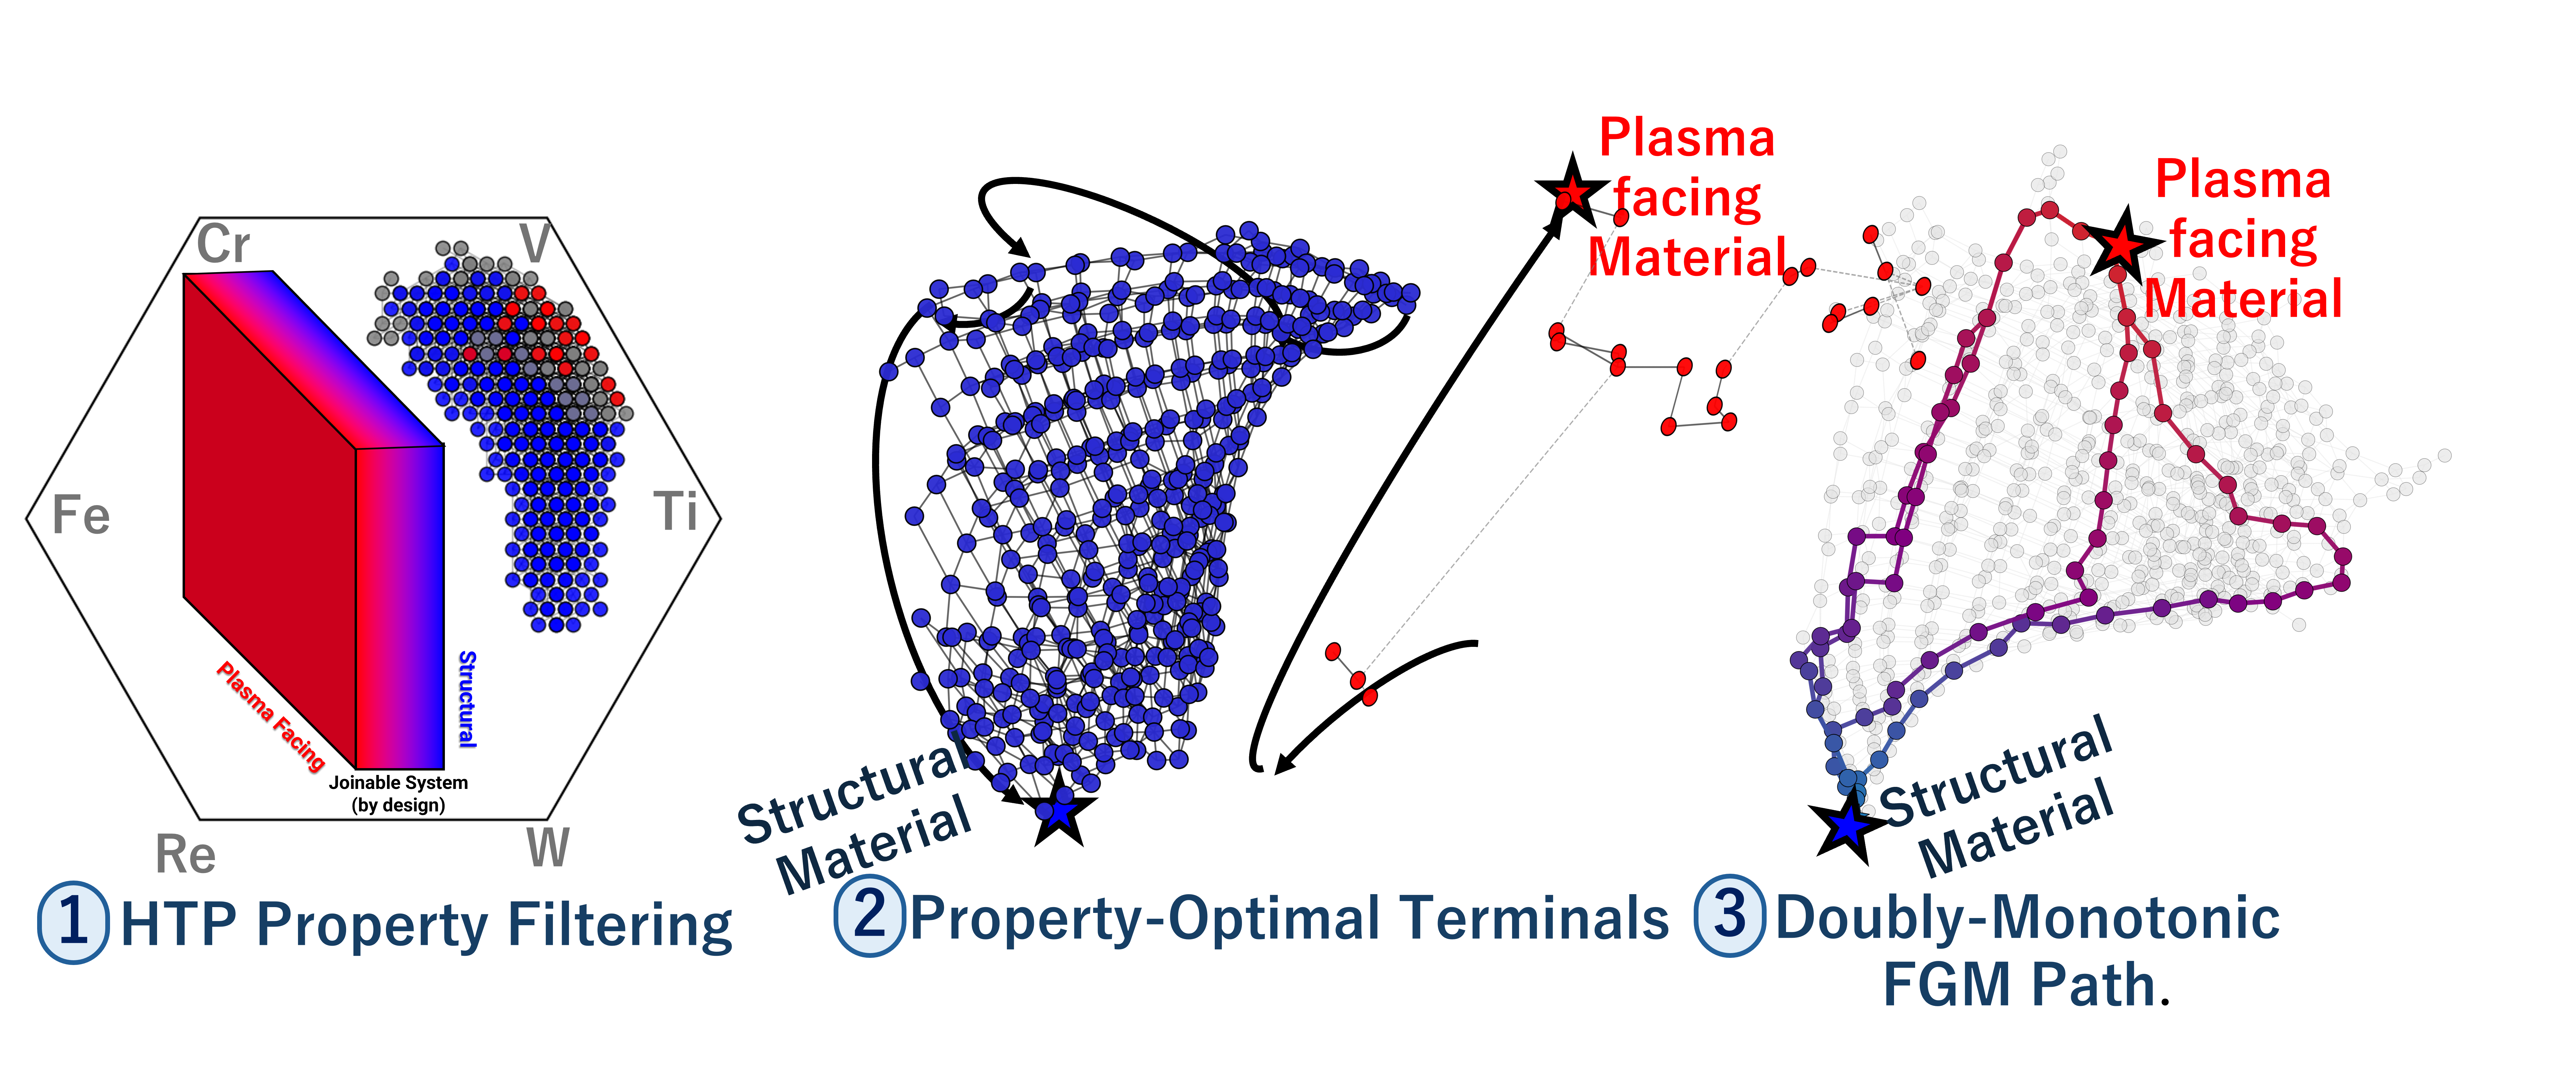
\includegraphics[width=0.9\textwidth]{figures/FGM-SCHEMATIC.png}
 \caption{Overview of the design workflow: property filtering of the
activation-feasible composition space, selection of the plasma-facing and
structural terminals, and doubly-monotonic graded-path design.}
  \label{fig:overview}
\end{figure*}
\section{Methods}
\subsection{Linear Programming Framework}
Linear programming (LP) provides a mathematical framework for solving
optimization and feasibility problems subject to linear constraints. In the
present work, LP is used to reformulate activation screening as a feasibility
problem in composition space. Rather than generating candidate alloy compositions
and subsequently evaluating whether they satisfy prescribed activation criteria,
the activation criteria are expressed directly as constraints on alloy
composition. The set of compositions satisfying all constraints defines a
feasible region within the atomic-fraction simplex. This reformulation shifts the
focus from evaluating individual compositions to constructing and exploring the
admissible region of composition space itself.

The applicability of LP to the present problem arises from the linear dependence
of FLARE activation responses on alloy composition. As a result, the activation
criteria can be expressed as a system of linear inequalities whose solution set
forms a convex polytope. The geometry of this feasible space can be characterized
analytically through vertex enumeration, while feasible alloy compositions can be
obtained through LP-guided exploration of the polytope. The framework therefore
replaces conventional generate-and-filter screening with a constraint-first
methodology that directly identifies compositions satisfying the prescribed
activation requirements.
\subsubsection{Alloy design domain and FLARE response model}
The alloy design domain considered in this work consists of the eleven-element
refractory system comprising Ti, V, Ta, Nb, Mo, Zr, Cr, Hf, Fe, Re, and W. An
alloy is represented by its atomic-fraction vector
\(x=(x_1,\ldots,x_N)\) with \(N=11\), where \(x_i\) is the atomic fraction of
element \(i\). Physically admissible compositions lie on the standard
\((N-1)\)-simplex,

\[
\Delta=\Big\{x\in\mathbb{R}^{N}:\sum_i x_i=1,\; x_i\ge0\Big\}, \tag{1}
\]

and the discrete design domain is the regular 5 at.% grid on \(\Delta\), i.e.,
the set of compositions whose fractions are integer multiples of 0.05. On an
eleven-element simplex, this grid contains approximately \(3\times10^7\)
compositions, illustrating the computational burden associated with conventional
generate-and-filter screening.

Candidate alloys are screened on their neutron-activation response using the
FLARE reduced-order model. FLARE computes each activation response of an alloy as
a composition-weighted sum of pre-tabulated pure-element contributions, so that
every response is linear in alloy composition. Responses are evaluated at a
neutron flux of \(8.0\times10^{13}\), an irradiation time of 2 years, and the
decay times associated with each screening criterion.

Screening is performed using five activation responses: gas production
\(M_{\mathrm{GAS}}\), total heat output \(HT_T\), and displacement damage
\(DPA\) at a decay time of approximately 1 s, together with contact dose rate
\(DOSE\) at decay times of 1 month and 100 years. Each response combines from its
per-element contributions in the appropriate extensive basis -- by weight
fraction for the mass-extensive responses (\(M_{\mathrm{GAS}}\), \(HT_T\), and
\(DOSE\)) and by atomic fraction for the atom-extensive response (\(DPA\)). This
distinction determines the exact form of the linear constraints constructed in
Section 2.1.2. Activation thresholds are defined relative to pure W and EUROFER97
reference response vectors, as described in the LP formulation of the following
section.
\subsubsection{LP constraint construction}
\subsubsection{Feasible polytope and vertex enumeration}
\subsubsection{LP-guided composition enumeration}





% Results and Discussion section.
% \ref{sec:results} is the target of the validation sentence in the methods section.
% Filter thresholds below are taken verbatim from the downstream-filter notebook.

\begin{figure*}[!b]
  \centering
  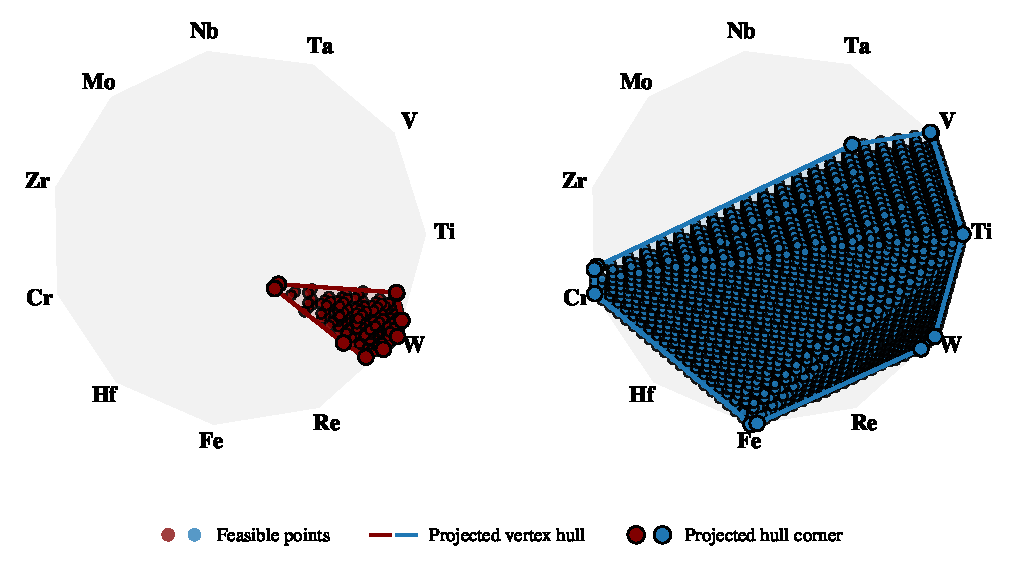
\includegraphics[width=0.90\textwidth]{figures/LP-FLARE-polytope-5at-10x.pdf}
  \caption{Activation-feasible compositions from the LP screen, projected onto the
eleven-element composition simplex. The left panel shows the \(10\times\)W
feasible region, and the right panel the \(10\times\)EUROFER97 region, with feasible
compositions as points and the projected vertex hull outlined.}
  \label{fig:polytope}
\end{figure*}

\section{Results and Discussion}
\label{sec:results}

\subsection{Feasible Space and Neutronic Screening}
\label{subsec:feasible}
Sampling of an eleven-element Cr-Fe-Hf-Mo-Nb-Re-Ta-Ti-V-W-Zr alloy
space on a \(5\)~at.\% grid yields \(30{,}045{,}015\) candidate
compositions, and evaluating every candidate individually at this scale
is costly. Since the activation responses are linear
in composition, the feasible region is instead constructed directly as a
polytope from the constraints, and the grid compositions lying inside it are
enumerated, producing \(210\) feasible compositions under the
\(10\times\)W reference and \(61{,}297\) under \(10\times\)EUROFER97.
The two feasible regions are shown projected onto the composition simplex in Fig.\ref{fig:polytope}. The two orders of magnitude
difference between the two sets reflects the baseline responses of the
references, since ten times a lower baseline is the tighter bound.
Although all eleven elements were free to vary, only Ti, V, Zr, Cr, Fe, Re, and W occur in the feasible compositions of either screen. The remaining four elements, Ta, Nb, Mo, and Hf, are excluded entirely by the activation criteria rather than by any prior restriction. By construction, every surviving composition remains within a factor
of ten of its reference material for all activation responses under the
irradiation conditions of Table~\ref{tab:ind_variables}, and this bound is retained through
the subsequent property screens.

The constraint-first approach was verified against a brute-force FLARE
evaluation of the full grid, which returned the same feasible compositions
under each reference, with every response agreeing to numerical precision.
The two approaches reach this result with different effort. The polytope
enumeration, which touches only the feasible set, completed in
\textcolor{red}{\texttt{Insert Runtime}}, while brute force evaluates every
grid candidate explicitly and becomes rapidly more expensive as the grid
grows. The deviation factor remains a tunable setting, and stricter or looser
values than the tenfold tolerance used here would contract or expand the
space accordingly, since the constraint bounds scale directly with it.


\subsection{Property Screening and Feasible Subgraphs}
\label{subsec:subgraphs}

For subgraph selection, the activation-feasible alloys identified in
Section~\ref{subsec:feasible} were evaluated with CALPHAD for phase stability and thermal
conductivity. The alloys from the two screens were merged into a single set, and
the \(204\) duplicated compositions were removed, leaving \(61{,}298\)
unique compositions. A candidate alloy is retained when its BCC phase fraction is at least $0.98$ at $500$, $600$, and $650\,^{\circ}\mathrm{C}$, keeping it single-phase, and when its room-temperature thermal conductivity exceeds $16~\mathrm{W/(m\cdot K)}$ for efficient heat transport. Applying both criteria together leaves $700$ compositions, representing $1.1\%$ of the $61{,}298$ candidate alloys, concentrated in the \ch{W-V-Cr-Fe} region of the simplex.


The connectivity of these (700) compositions after applying the two constraints is shown in Fig.~\ref{fig:clusters}, forming three disconnected subgraphs. Subgraph~1 contains (686) compositions, about (98\%) of the survivors, and forms a connected region spanning the \ch{W-V-Cr-Fe} band from the tungsten-rich corner to the vanadium- and titanium-rich region. Subgraphs~2 and~3 are small isolated islands of eight and six compositions, feasible in every screened property yet unreachable from Subgraph~1. A path within a subgraph moves between compositions in small steps without leaving the feasible set, whereas crossing between subgraphs would require passing through infeasible compositions. Subgraph~1, offering the largest contiguous space for a graded transition, is therefore carried forward as the design region for the graded alloy.


\begin{figure}[H]
  \centering

\includegraphics[width=0.75\linewidth]{manuscript/figures/LP_FLARE_nim_fig1_all_subgraphs.pdf}
 \caption{Feasible compositions in the eleven-element design space after neutronics,
phase, and thermal-conductivity screening.}
  \label{fig:clusters}
\end{figure}

%The combined feasible set, comprising the survivors of both the \(10\times\)W and\(10\times\)EUROFER97 screens, is next evaluated for its thermodynamic and thermophysical properties by CALPHAD and subjected to fusion-relevant property constraints in two stages. The \(204\) compositions feasible under both references were equilibrated in both screening passes and thus serve as replicate calculations: \(199\) agree to within \(1\)~K in solidus, mutually validating the CALPHAD inputs, while the remaining five, tungsten-rich compositions bearing Fe and Re, disagree beyond tolerance and are excluded as non-converged equilibria, leaving \(61{,}298\) unique compositions for property screening. The first stage applies two universal requirements, a stable single-phase BCC structure, taken as a maximum BCC mole fraction of at least \(0.98\) at \(500\), \(600\), and \(650\,^{\circ}\mathrm{C}\), and a room-temperature thermal conductivity above \(16\)~W/(m\,K), selecting for phase stability across the operating range and for adequate heat removal.

%\begin{figure}[H]
  %\centering
%
\includegraphics[width=0.75\linewidth]{manuscript/figures/LP_FLARE_nim_fig1_all_subgraphs.pdf}
 %\caption{Feasible compositions in the eleven-element design space after neutronics,
%CALPHAD, and thermal-conductivity screening. Subgraph~1 (blue) represents the largest connected set, suitable for FGM development.}
  %\label{fig:clusters}
%\end{figure}

%To group the surviving compositions, those passing the BCC and conductivity filters are connected into a traversal graph on the composition lattice: each feasible composition is a node, and two nodes share an edge when they differ by a single \(5\)~at.\% exchange between two elements, following the simplex-lattice adjacency of NIMPLEX~\cite{nimplex}. The connected components of this graph are the feasible subgraphs (Figure~\ref{fig:clusters}). This grouping has a direct physical meaning, since a path within a single component moves between compositions in small steps without leaving the feasible set, whereas crossing between components would require passing through infeasible compositions~\cite{nimplex}. Of the \(700\) compositions surviving both filters, three components result: a large subgraph of \(686\) compositions spanning the \ch{W-V-Cr-Fe} band and two much smaller, genuinely isolated islands of \(8\) and \(6\) compositions, feasible in every property yet unreachable from the main region by any single \(5\)~at.\% step. The largest, being the most connected region of the feasible set, is the natural candidate for a graded plasma-facing-to-structural material and is carried forward.



\subsection{Plasma-Facing and Structural Alloy Classification}

The \(686\) compositions of Subgraph~1 were classified according to
two design targets, a solidus temperature above
\(2200\,^{\circ}\mathrm{C}\) for high-temperature capability and a Pugh
ratio of \(2.6\) for intrinsic ductility. Compositions meeting the solidus requirement are designated Alloy~A
and are the plasma-facing material (PFM) candidates, and those meeting the
ductility requirement are designated Alloy~B, the structural candidates.
Compositions meeting both requirements are designated Alloy~AB, and these
satisfy the demands of both sides and serve as a bridge between the
plasma-facing and structural regions. The remaining compositions, which meet
neither requirement, are designated Intermediate and are not considered in
the terminal selection, although they remain part of the traversable design
region. Of these, \(148\) qualify as
Alloy~A, \(353\) as Alloy~B, \(18\) as Alloy~AB, and \(167\) are
Intermediate. Their distribution across the simplex is shown in
Figure~\ref{fig:categories}, where Alloy~A clusters in the tungsten-rich
corner and Alloy~B in the vanadium-rich region. The
two-property classification thus identifies the plasma-facing and structural
materials within the design region, with the small Alloy~AB set lying
between them and reconciling high-temperature capability with intrinsic
ductility.

\begin{figure}[H]
  \centering
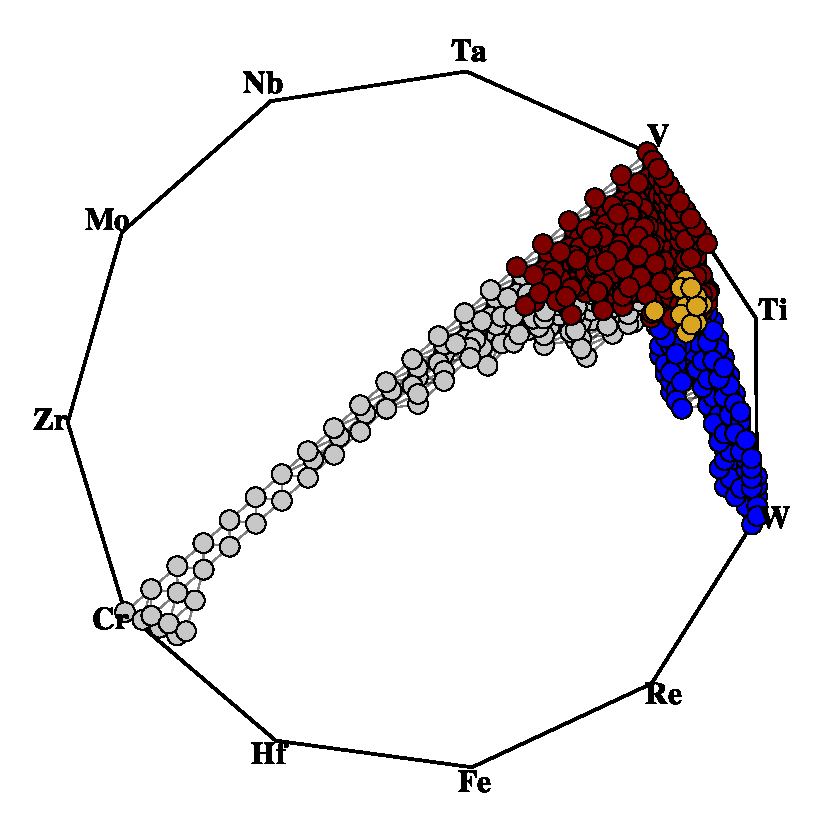
\includegraphics[width=0.75\linewidth]{figures/LP_FLARE_nim_fig2_subgraph1_categories.pdf}
\caption{Candidate categories of Subgraph~1 on the composition simplex,
with Alloy~A in blue, Alloy~B in maroon, Alloy~AB in goldenrod, and
Intermediate in grey.}
  \label{fig:categories}
\end{figure}

Fig.~\ref{fig:properties} maps the two classification properties
over Subgraph~1, with the Pugh ratio in panel~(a) and the solidus
temperature in panel~(b). The two maps display opposite gradients. The Pugh
ratio increases from the tungsten-rich corner toward the vanadium-rich compositions, while the solidus temperature peaks in the
tungsten-rich corner and falls in the direction the ductility rises, so that
the two properties are strongly anticorrelated across the subgraph. The
subgraph therefore spans a continuous trade-off between high-temperature
capability and ductility, and the maps locate where each design target is
met, with the plasma-facing candidates at one end and the structural
candidates at the other. The graded-path design of the next section is built on this classified region.

\label{subsec:classification}
\begin{figure*}[b]
  \centering
  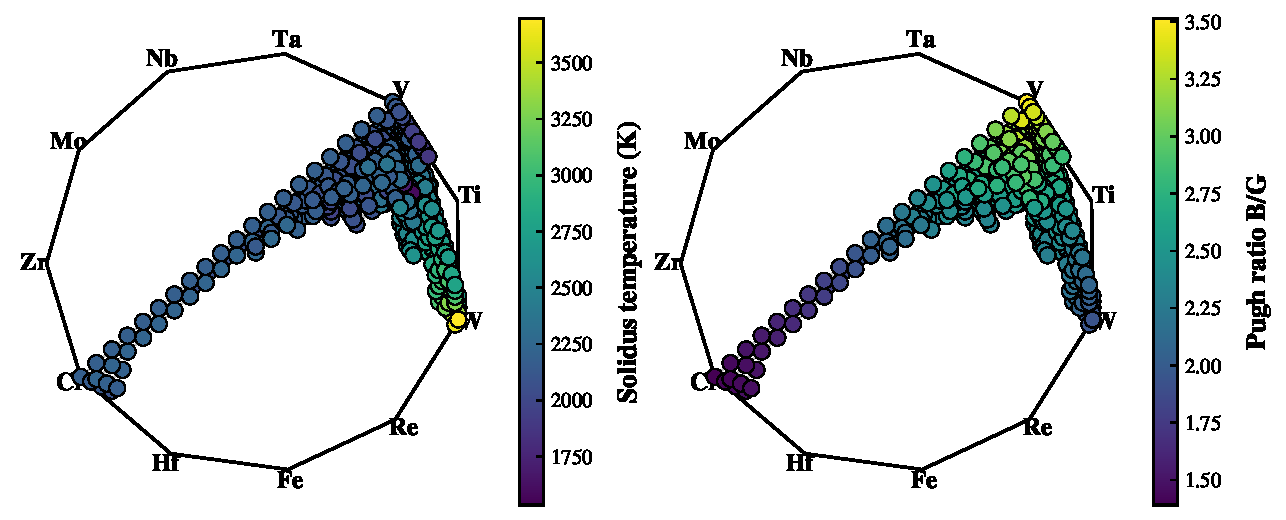
\includegraphics[width=0.80\textwidth]{figures/LP_FLARE_nim_fig3_subgraph1_properties.pdf}
  \caption{CALPHAD properties across the largest connected subgraph, projected
  onto the composition simplex: (a) Pugh ratio (\(B/G\)) and (b) solidus
  temperature.}
  \label{fig:properties}
\end{figure*}


\subsection{Doubly-Monotonic Path Planning}
\label{subsec:path}
The design question is whether the two regions identified in
Section~\ref{subsec:classification} can be joined by a compositional
gradient whose properties evolve in one direction only, so that no interior
layer of the graded wall is hotter-melting than the layer in front of it or
less ductile than the layer behind it. This is posed as a path problem on the traversal graph of
Subgraph~1, with terminals restricted to deployable multi-component alloys
of at least three constituents and no single element above \(90\)~at.\%.
Without this restriction, the property extrema are the pure elements, and the
design degenerates to a trivial W\(\to\)V elemental gradient anchored by
non-deployable terminals. Within the deployable pools (\(147\) plasma-facing
and \(342\) structural candidates), the plasma-facing terminal is taken as
the maximum-solidus composition among the Alloy~A and AB candidates and the
structural terminal as the maximum-Pugh composition among the Alloy~B and AB
candidates. Monotonicity is enforced as a hard constraint by removing from the
traversal graph every directed edge that raises the solidus or lowers the
Pugh ratio, after which Dijkstra's algorithm returns the exact shortest path
on what remains. The search objective is unweighted path
length, so the formulation contains no tuning parameters, in contrast to
penalized cost-function approaches in which monotonicity is promoted through a
weight that must be selected~\cite{kirk2021monotonic}.


The resulting terminals are V\(_{5}\)Re\(_{5}\)W\(_{90}\) (solidus
\(3449\)~K) for the plasma-facing role and Ti\(_{5}\)V\(_{90}\)Re\(_{5}\)
(Pugh ratio \(3.34\)) for the structural role. A strict doubly-monotonic path
between them exists, consisting of \(19\) alloys connected by \(18\) steps of
a single \(5\)~at.\% exchange each, along which the solidus never rises and
the Pugh ratio never falls from one step to the next, verified independently
by per-step assertion and by a loss-of-invariance metric of zero for both
properties (Figures~\ref{fig:path} and~\ref{fig:path-profiles}). At each
step, \(5\)~at.\% of one element is exchanged for another, the smallest
possible move between neighboring compositions on the design grid. Every
intermediate composition on the path satisfies the activation,
phase-stability, and conductivity screens by construction. Eighteen
steps is also the minimum conceivable for this terminal pair, since
the tungsten content alone must change by eighteen lattice units, so the
monotonicity requirement is achieved at zero cost in path length. The pruned
formulation, in which only \(2{,}030\) of the \(7{,}348\) directed
transitions in Subgraph~1 survive, guarantees this by construction, as any
shortest path on the pruned graph is monotone.

\begin{figure}[H]
  \centering
  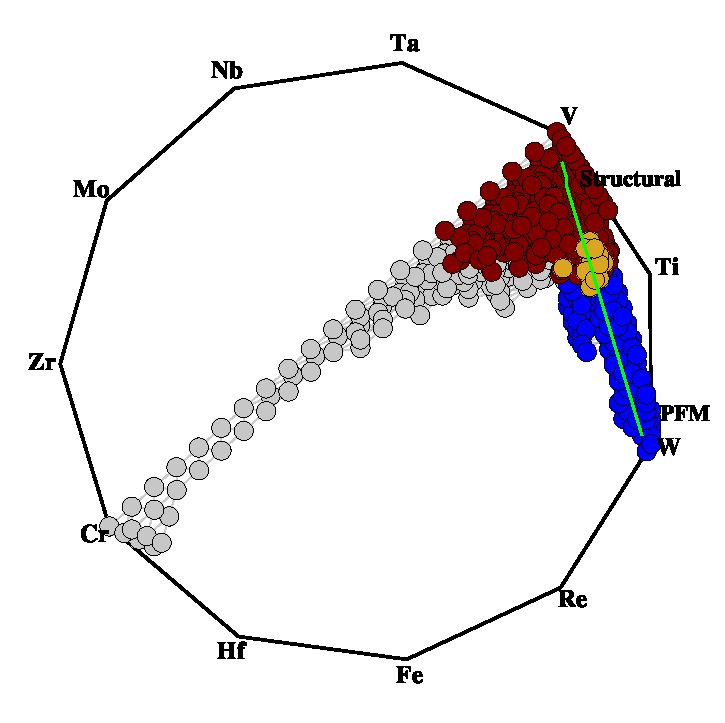
\includegraphics[width=0.8\linewidth]{figures/LP_FLARE_nim_fig6_graded_path.pdf}
  \caption{The shortest doubly-monotonic path (green) across the
classified compositions of Subgraph~1, from the PFM terminal to the
structural terminal on the composition simplex.
Node colors follow Figure~\ref{fig:categories}.}
  \label{fig:path}
\end{figure}

Fig.~\ref{fig:path-profiles} shows the property evolution along
this route. The solidus falls from \(3449\) to
\(2195\)~K and the Pugh ratio rises from \(2.00\) to \(3.34\), with the
largest solidus drops concentrated in the tungsten-rich early steps and the
largest ductility gains toward the vanadium-rich end. The two curves cross
their respective category thresholds within the Alloy~AB window, at steps 10 to 12 of the path.

\begin{figure}[H]
  \centering
  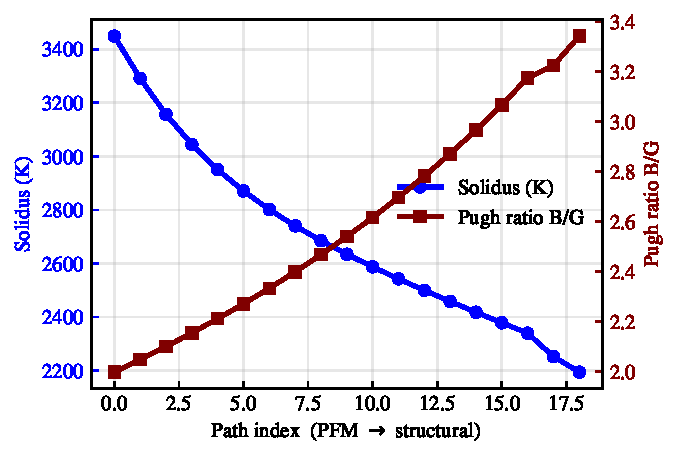
\includegraphics[width=1\linewidth]{figures/LP_FLARE_nim_fig7_path_property_profile.pdf}
  \caption{Solidus temperature and Pugh ratio along the path, from the
plasma-facing terminal (index~0) to the structural terminal (index~18). The
solidus is non-increasing and the Pugh ratio non-decreasing at every step.}
  \label{fig:path-profiles}
\end{figure}

The \(18\) Alloy~AB compositions prove structurally essential to this result.
A connectivity test on the pruned graph shows that no doubly-monotonic
route exists between the terminals when these compositions are removed, as
every admissible route from the plasma-facing candidates to the structural
candidates is forced through the dual-criteria class, and the optimal path
traverses three of its eighteen members. The overlap of the two property criteria is
therefore not incidental but constitutes the sole monotone gateway between
the plasma-facing and structural categories. To our knowledge, enforcing monotonicity in two
opposing properties simultaneously has not been reported in the
compositionally graded alloy path-planning literature, which has treated
monotonicity in a single property~\cite{kirk2021monotonic}. The
complete path is given in Table~\ref{tab:path}, traversing the Alloy~A, AB,
and B categories in sequence.

\begin{table*}[!t]
\centering
\caption{The shortest doubly-monotonic graded path: nineteen alloys connected by
eighteen steps of a single 5~at.\% exchange each, from the plasma-facing terminal
(index~0) to the structural terminal (index~18). The solidus is non-increasing
and the Pugh ratio non-decreasing at every step; the three Alloy~AB compositions
(indices 10-12) constitute the monotone gateway between the two categories.}
\label{tab:path}
\begin{tabular}{clllcc}
\toprule
Index & Composition (at.\%) & Step & Solidus (K) & Pugh $B/G$ & Category \\
\midrule
0 & V$_{5}$Re$_{5}$W$_{90}$ & -- & 3449 & 2.00 & A \\
1 & V$_{10}$Re$_{5}$W$_{85}$ & W\,$-5$, V\,$+5$ & 3292 & 2.05 & A \\
2 & V$_{15}$Re$_{5}$W$_{80}$ & W\,$-5$, V\,$+5$ & 3157 & 2.10 & A \\
3 & V$_{20}$Re$_{5}$W$_{75}$ & W\,$-5$, V\,$+5$ & 3045 & 2.15 & A \\
4 & V$_{25}$Re$_{5}$W$_{70}$ & W\,$-5$, V\,$+5$ & 2951 & 2.21 & A \\
5 & V$_{30}$Re$_{5}$W$_{65}$ & W\,$-5$, V\,$+5$ & 2871 & 2.27 & A \\
6 & V$_{35}$Re$_{5}$W$_{60}$ & W\,$-5$, V\,$+5$ & 2802 & 2.33 & A \\
7 & V$_{40}$Re$_{5}$W$_{55}$ & W\,$-5$, V\,$+5$ & 2741 & 2.40 & A \\
8 & V$_{45}$Re$_{5}$W$_{50}$ & W\,$-5$, V\,$+5$ & 2686 & 2.47 & A \\
9 & V$_{50}$Re$_{5}$W$_{45}$ & W\,$-5$, V\,$+5$ & 2635 & 2.54 & A \\
10 & V$_{55}$Re$_{5}$W$_{40}$ & W\,$-5$, V\,$+5$ & 2588 & 2.62 & AB \\
11 & V$_{60}$Re$_{5}$W$_{35}$ & W\,$-5$, V\,$+5$ & 2543 & 2.70 & AB \\
12 & V$_{65}$Re$_{5}$W$_{30}$ & W\,$-5$, V\,$+5$ & 2500 & 2.78 & AB \\
13 & V$_{70}$Re$_{5}$W$_{25}$ & W\,$-5$, V\,$+5$ & 2459 & 2.87 & B \\
14 & V$_{75}$Re$_{5}$W$_{20}$ & W\,$-5$, V\,$+5$ & 2418 & 2.97 & B \\
15 & V$_{80}$Re$_{5}$W$_{15}$ & W\,$-5$, V\,$+5$ & 2379 & 3.07 & B \\
16 & V$_{85}$Re$_{5}$W$_{10}$ & W\,$-5$, V\,$+5$ & 2340 & 3.18 & B \\
17 & Ti$_{5}$V$_{85}$Re$_{5}$W$_{5}$ & W\,$-5$, Ti\,$+5$ & 2253 & 3.23 & B \\
18 & Ti$_{5}$V$_{90}$Re$_{5}$ & W\,$-5$, V\,$+5$ & 2195 & 3.34 & B \\
\bottomrule
\end{tabular}
\end{table*}



Fig.~\ref{fig:path-composition} shows the compositional simplicity
of the path. Tungsten declines and vanadium rises together across sixteen
consecutive exchanges, rhenium remains a constant \(5\)~at.\% from terminal
to terminal, and titanium enters only in the final two layers as the tungsten
is exhausted. Although the path was searched
in an eleven-element space, it engages only four elements, and at no point do
more than four coexist. In practical terms, the entire gradient can be
deposited from two varying feed streams against a constant rhenium addition,
with a single titanium introduction near the structural end


\begin{figure}[H]
  \centering
  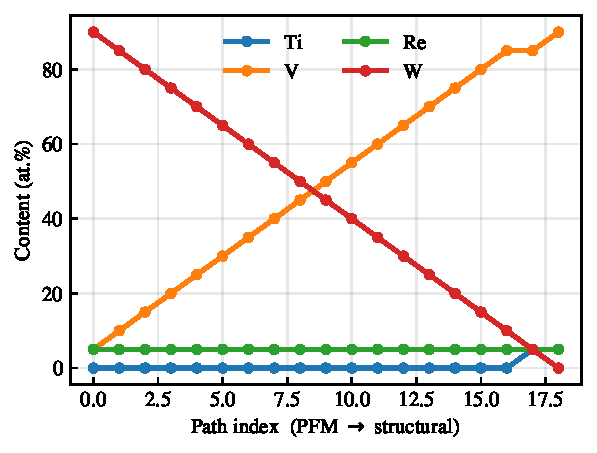
\includegraphics[width=0.9\linewidth]{figures/LP_FLARE_nim_fig8_path_composition_profile.pdf}
  \caption{Elemental composition along the path: a tungsten-vanadium
substitutional gradient at constant 5~at.\% Re, with Ti introduced in the
final two layers as W is exhausted. Each step changes exactly one element pair
by 5~at.\%.}
  \label{fig:path-composition}
\end{figure}


\subsection{ELM Assessment of the Graded Design}
\label{subsec:elm}

As a final assessment, the graded design is evaluated against transient
edge-localized-mode (ELM) heat loading, the surface requirement that the
equilibrium screens do not address. The assessment was carried out over all
\(686\) compositions of Subgraph~1, so that the melting capability of the
entire classified region is established rather than that of the path alone.
For each composition, the peak surface temperature during an ELM pulse was
computed from its CALPHAD-derived thermal properties
(Section~\ref{subsec:elm-methods}), and the ELM melting margin was defined
as the alloy solidus minus this peak temperature, so that a positive margin
means the surface stays below melting.

Fig.~\ref{fig:elm} shows the margin across the classified region. It
ranges from \(-4140\) to \(+2229\)~K with a mean of \(-806\)~K, and \(114\)
of the \(686\) compositions (\(17\%\)) remain positive. The margin
correlates strongly with tungsten content, the passing compositions
averaging \(57\)~at.\% W against \(12\)~at.\% W for those that fail, since
tungsten raises the solidus that the surface temperature is measured
against. The ELM-resistant set is not limited to near-pure
tungsten. Tungsten alloyed with Ti, V, and Re retains a positive margin, and
a small group of Cr-rich compositions also passes, eight of the thirty-one
with at least \(50\)~at.\% Cr, so several compositional routes to ELM
resistance exist within the region. The pass/fail boundary is sharp, with
\(76\) compositions lying within \(\pm200\)~K of zero margin.

\begin{figure*}[!t]
  \centering
  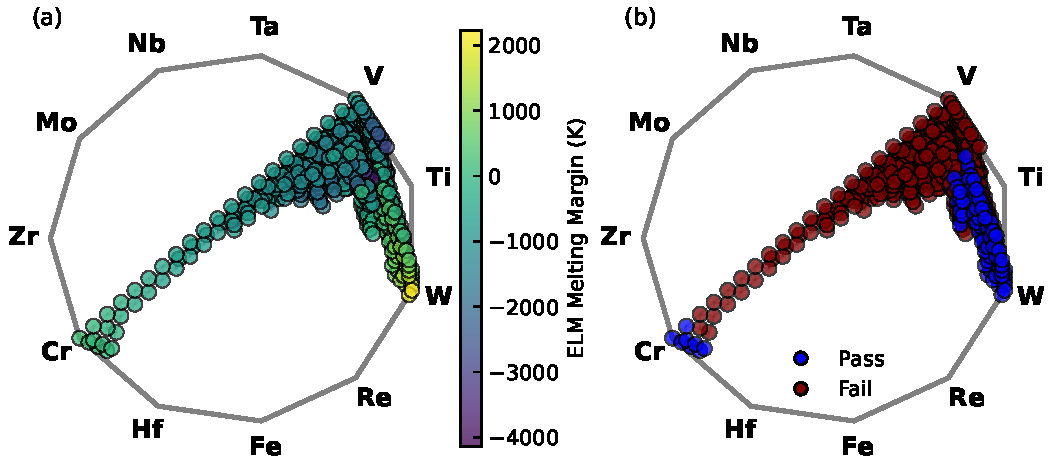
\includegraphics[width=0.80\textwidth]{figures/LP-FLARE-ELM-margin-panels.pdf}
  \caption{ELM assessment across the largest connected subgraph, projected
onto the composition simplex: (a) ELM melting margin and (b) the resulting
pass/fail classification, with blue marking compositions of positive margin
(pass) and maroon those of negative margin (fail).}
  \label{fig:elm}
\end{figure*}

The graded path passes this test exactly where it must. Its plasma-facing
terminal, V\(_{5}\)Re\(_{5}\)W\(_{90}\), carries a margin of \(+1650\)~K,
placing it comfortably within the ELM-resistant set, and the margin
decreases smoothly along the path, remaining positive through the first
twelve layers, the entire Alloy~A segment and two of the three gateway
compositions before crossing zero at the transition into the structural
category. The ELM-resistant extent of the gradient therefore coincides with
its plasma-facing function, as the layers that face the plasma withstand the
transient while the structural layers behind them, shielded from surface
loading, are not required to. The ELM assessment thus adds a third,
independent line of evidence that converges with the activation and
mechanical screens on the same separation of plasma-facing and structural
materials, now traced layer by layer along the designed gradient.
\section{Conclusion}
This work designed a functionally graded alloy for the fusion first wall as a
doubly monotonic path through an eleven-element refractory composition space.
The design proceeds in four stages. Activation screening referenced to pure
tungsten and to EUROFER97 exploits the linearity of the FLARE responses, so
that the feasible space is obtained by linear programming without evaluating
the more than thirty million rejected candidates. CALPHAD-based property
filtering then enforces single-phase BCC stability and thermal conductivity,
a traversal graph is constructed on the surviving compositions, and the
shortest path is found under monotonicity imposed as a hard constraint, by
deleting every transition that raises the solidus or lowers the Pugh ratio
before an exact search. Of the
\(61{,}298\) unique activation-feasible compositions, \(700\) survive
the property screens, \(686\) of them forming a single connected design
region in which high-solidus plasma-facing candidates and ductile structural
candidates occupy opposite ends of a continuous trade-off. Between deployable
terminals, V\(_{5}\)Re\(_{5}\)W\(_{90}\) and Ti\(_{5}\)V\(_{90}\)Re\(_{5}\),
a strict doubly-monotonic path of nineteen alloys exists, a
tungsten-vanadium substitutional gradient at constant \(5\)~at.\% Re in
which the solidus only decreases, from \(3449\) to \(2195\)~K, and the Pugh
ratio only increases, from \(2.00\) to \(3.34\), at every one of its eighteen
single-exchange steps. The path length equals the minimum possible for these
terminals, so the monotonicity requirement is achieved at zero cost, and the
eighteen compositions satisfying both design criteria prove to be the sole
monotone gateway between the two categories, the path crossing three of
them. An edge-localized-mode assessment independently validates the design,
with the plasma-facing terminal carrying a melting margin of \(+1650\)~K and
the margin remaining positive along the gradient precisely through its
plasma-facing extent, the structural layers behind it sitting shielded from
surface loading.

The formulation generalizes in both of its parts. The constraint-first
screening applies to any model whose responses are linear in composition, and
the hard-constraint path planning applies to any graded-alloy design
requiring monotonicity in one or more properties, with no tuning parameters
to select. Future work will pursue validation, realization, and
generalization through experimental characterization of the
descriptor-level properties along the path, synthesis of the terminal and
gateway compositions, a graded build to test the predicted through-wall
profile, and extension of the path formulation to multi-objective design, in
which path length is balanced against additional objectives such as
thermal-expansion mismatch or activation margin.
\section*{Code Availiability}

The code associated with this work is available at the following repository: 

\section*{Declaration of Generative AI and AI-assisted technologies in the writing process}

During the preparation of this work, the authors used GPT-4-turbo in order to ideate/brainstorm alternative sentence structures and stylistic choices in limited sections of the paper. After using this tool/service, the authors reviewed and edited the content as needed and take full responsibility for the content of the publication.
\input{07_competing-interest-decleration}
\section*{Acknowledgements}
We acknowledge the support from the U.S.~Department of Energy (DOE) ARPA-E ULTIMATE Program through Project DE-AR0001427. R.A.~also acknowledges the Army Research Laboratory (ARL) for support through Cooperative Agreement Number W911NF-22-2-0106, as part of the High-throughput Materials Discovery for Extreme Conditions (HTMDEC) program as supported by the BIRDSHOT Center at Texas A\&M University. B.V. acknowledges the support of NSF through Grant No.~1746932 (GRFP) and 1545403 (NRT-D3EM). R.A.~and D.S.~acknowledge support from the Army Research Office (ARO) through Grant No.~W911NF-22-2-0117. Portions of this research were conducted with the advanced computing resources provided by Texas A\&M High Performance Research Computing.
\section*{CRediT authorship contribution statement}
\textbf{Samuel Ifada}: Writing – original draft, Writing – review \& editing, Visualization, Software, Investigation, Formal analysis, Data curation. \textbf{Brent Vela}: Writing – original draft, Visualization, Software, Validation, Investigation, Formal analysis, Data curation. \textbf{Raymundo Arróyave}: Writing – review \& editing, Project administration, Funding acquisition. \textbf{Brent Vela}: Writing – original draft, Writing – review \& editing, Visualization, Software, Investigation, Formal analysis, Data curation, Conceptualization, Methodology, Supervision.

% Conceptualization
% Data curation
% Formal analysis
% Funding acquisition
% Investigation
% Methodology
% Project administration
% Resources
% Software
% Supervision
% Validation
% Visualization
% Writing – original draft
% Writing – review \& editing

\bibliographystyle{elsarticle-num}
\bibliography{ref}

\end{document}
